\documentclass[11pt,ignorenonframetext,aspectratio=169,xcolor={svgnames}]{beamer}
\usetheme{Szeged}
\usecolortheme{crane}
\usefonttheme{structurebold}
\usefonttheme{professionalfonts}
\usepackage{amssymb,amsmath}
\usepackage{ifxetex,ifluatex}
\usepackage{fixltx2e} % provides \textsubscript
\ifxetex
  \usepackage{fontspec,xltxtra,xunicode}
  \defaultfontfeatures{Mapping=tex-text,Scale=MatchLowercase}
\else
  \ifluatex
    \usepackage{fontspec}
    \defaultfontfeatures{Mapping=tex-text,Scale=MatchLowercase}
  \else
    \usepackage[utf8]{inputenc}
  \fi
\fi
\usepackage{listings}

% Comment these out if you don't want a slide with just the
% part/section/subsection/subsubsection title:
% \AtBeginPart{
%   \let\insertpartnumber\relax
%   \let\partname\relax
%   \frame{\partpage}
% }
% \AtBeginSection{
%   \let\insertsectionnumber\relax
%   \let\sectionname\relax
%   \frame{\sectionpage}
% }
% \AtBeginSubsection{
%   \let\insertsubsectionnumber\relax
%   \let\subsectionname\relax
%   \frame{\subsectionpage}
% }

\setlength{\parindent}{0pt}
\setlength{\parskip}{6pt plus 2pt minus 1pt}
\setlength{\emergencystretch}{3em}  % prevent overfull lines
\setcounter{secnumdepth}{0}

%%% begin dwr insert
\usepackage{patchcmd}
\usepackage{tabulary}   % Support longer table cells
\usepackage{booktabs}   % Support better tables
\usepackage[sort&compress]{natbib}

\usepackage{framed}     % Allow background color for images
\definecolor{shadecolor}{named}{white}

%\usepackage{paralist}
\usepackage{xparse}
\usepackage{subfigure}
\usepackage{hyperref}
%%% end dwr insert
\usepackage{rosoff-vector-macros}
\usepackage[beamer]{cofi}
\title{More practice with parametrizations}
\author{Math 275 Calculus 3}
\date{November 18, 2013}
%% begin.rcode setup, echo=FALSE, include=FALSE
% library(knitr)
% opts_chunk$set(out.width=6, out.height=6, dev='pdf')
%% end.rcode
\begin{document}
\frame{\titlepage}

\section{More practice with parametrizations}

% \begin{frame}\frametitle{Exam data}
% %% begin.rcode grades, echo=FALSE, include=FALSE
% % grades = c(47,56,57,58,60,60,62,65,66,68,68,73,74,75,76,76,76,78,81,82,82,83,83,84,84,87,88,89,92,95,96)
% %% end.rcode
% The average was $\rinline{mean(grades)}$ ($n = 31$) with $\sigma = \rinline{sd(grades)}$.
% \begin{figure}[ht]
% \begin{minipage}[m]{0.2\linewidth}
% \begin{tabular}{cr}
%     min & $\rinline{min(grades)}$ \\
%     Q1 & $\rinline{quantile(grades, 0.25)}$ \\
%     Q2 & $\rinline{quantile(grades, 0.50)}$ \\
%     Q3 & $\rinline{quantile(grades, 0.75)}$ \\
%     max & $\rinline{max(grades)}$
% \end{tabular}
% \end{minipage} \hspace*{1em} 
% \begin{minipage}[m]{0.6\linewidth}
% %% begin.rcode hist, echo=FALSE, include=FALSE
% % hist(grades)
% %% end.rcode
% 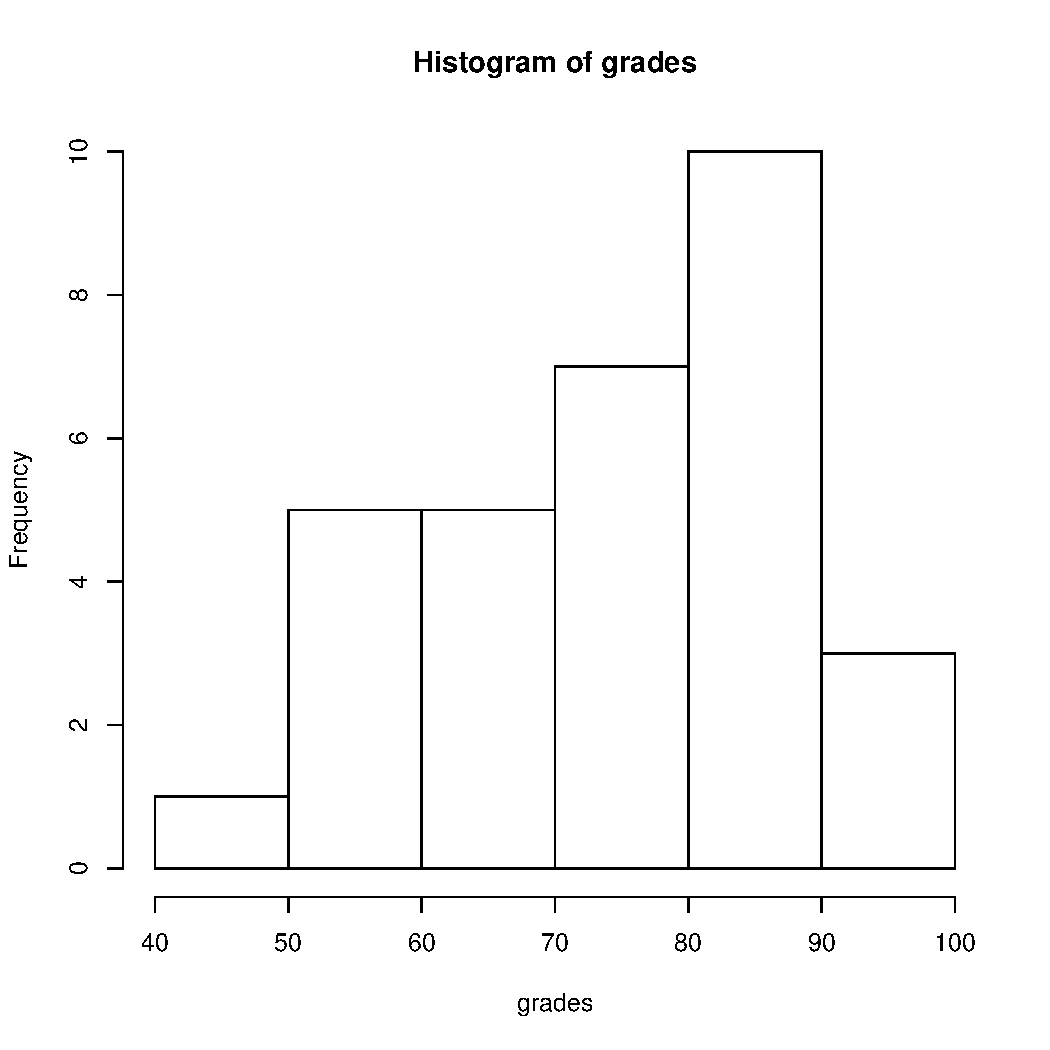
\includegraphics[width=0.8\textwidth, height=0.8\textwidth]{figure/hist.pdf}
% \end{minipage}
% \end{figure}

% \end{frame}

\begin{frame}\frametitle{Warm-up}

\emph{Gluing parametrizations}. Let $P$, $Q$, and $R$ be the points
$(1,0)$, $(0,1)$, and $(-1,0)$, respectively, and let $\gamma$ be the
V-shaped path joining $P$ to $Q$ and thence to $R$ via segments.

\begin{itemize}[<+->]
\itemsep1pt\parskip0pt\parsep0pt
\item
  Parametrize $\gamma$ in such a way that $\gamma(0) = P$ and
  $\gamma(2) = R$.
\item
  Answer: $\vec{r}(t) = \angl{1-t, t}$ if $0 \leq t \leq 1$ and
  $\vec{r}(t) = \angl{1-t, 2-t}$ if $1 \leq t \leq 2$.
\end{itemize}

\end{frame}

\begin{frame}\frametitle{Tangent vectors, velocity, speed, and
arclength}

If $\vec{r}(t)$ is a vector function, we say it is continuous if all its
entries are continuous functions. Same thing for differentiable. We
think of $\vec{r}(t)$ as a position function, because at each time $t$
it shows how to get to our particle from the origin. Then its derivative
$\vec{r}'(t)$ turns out to be the instantaneous velocity vector of the
moving particle.

\begin{itemize}[<+->]
\itemsep1pt\parskip0pt\parsep0pt
\item
  If exactly at time $t$ you detach the moving particle from the
  function $\vec{r}$ and let it move in the exact direction and speed it
  had at that moment, then at time $t+1$ it has moved by exactly
  $\vec{r}'(t)$.
\item
  How do we differentiate? One entry at a time.
  $\vec{r}'(t) = \angl{x'(t), y'(t)}$ and so on.
\end{itemize}

\end{frame}

\begin{frame}\frametitle{Velocity as a vector}

Velocity has always been a vector. You know that speed is nonnegative,
while in one dimension velocity carries a sign. This is information
about the direction of travel, just as meaningful as the speed itself.
Since motion in a plane isn't confined to a backward and a forward
direction, we need the complete generality of vectors in the plane to
describe the possible velocities a moving particle might have.

Usually, when we draw parametrized curves, we don't actually draw the
vectors $\vec{r}(t)$. Instead we draw the trajectory: the collection of
endpoints of $\vec{r}(t)$. But we frequently will draw the vector
$\vv(t) = \vec{r}'(t)$ attached to the curve, with its tail at the
endpoint of $\vec{r}(t)$. It's a moving tangent vector!

\end{frame}

\begin{frame}\frametitle{Speed as the length of velocity}

The entries of the velocity vector (tangent vector---same thing) tell
you the velocities in each of the coordinate directions. But the speed
is something else. It is the magnitude of the velocity vector. In two
dimensions,

\begin{equation*}
    \frac{ds}{dt} = \norm{\angl{x'(t), y'(t)}} = \sqrt{x'(t)^2 + y'(t)^2}
\end{equation*}

\end{frame}

\begin{frame}\frametitle{Arc length}

We can obtain the length of a parametrized curve (not the same thing as
the length of its time domain or parameter interval) by integrating
speed over the parameter interval $[a,b]$:

\begin{equation*}
    s = \int_a^b \frac{ds}{dt} \; dt = \int_a^b \sqrt{\left( \frac{dx}{dt} \right)^2 + \left( \frac{dy}{dt} \right)^2} \; dt
\end{equation*}

\end{frame}

\begin{frame}\frametitle{Practice translating, scaling, gluing}

\begin{itemize}
\itemsep1pt\parskip0pt\parsep0pt
\item
  Circle, center at origin, traced once counterclockwise, starting at
  $(0,3)$ with $t \in [0,1]$.
\item
  Circle, center at $(a,b)$, traced once counterclockwise, starting at
  $(a+r, b)$ with $t \in [0, 2\pi] = [0, \tau]$.
\item
  Circle, center at origin, traced once \emph{clockwise}, starting at
  $(1,0)$.
\item
  Pseudotriangle with boundary the segments from $(0,1)$ to $(0,0)$,
  from $(0,0)$ to $(1,0)$, and the arc of the unit circle connecting
  $(1,0)$ to $(0,1)$. Traverse counterclockwise with time interval
  $[0,1]$.
\end{itemize}

\end{frame}

\end{document}
